To show that $\mathbf{AFG}~p$ is not equivalent to $\mathbf{AFAG}~p$ we
construct a Kripke structure which contains a state where $\mathbf{AFG}~p$
holds but $\mathbf{AFAG}~p$ does not.
Figure~\ref{figure:Kripke_Structure_Exercise_6}~\cite{Veith2011ExerciseSolutions} shows this Kripke structure
, where $s₀⊧\mathbf{AFG}~p$ holds, but
$s₀⊧\mathbf{AFAG}~p$ does not.

\begin{figure}[htbp]
    \centering
        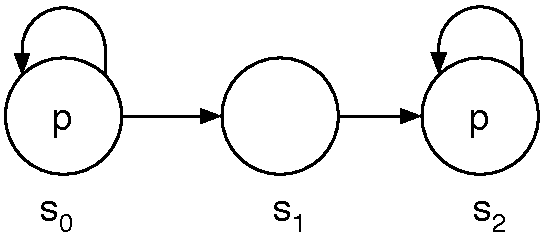
\includegraphics[width=.4\textwidth]
            {Figures/Kripke Structure Exercise 6.pdf}
    \caption{Kripe Structure, where $s₀⊧\mathbf{AFG}~p$ holds, but
             $s₀⊧\mathbf{AFAG}~p$ does not hold}
    \label{figure:Kripke_Structure_Exercise_6}
\end{figure}

\begin{figure}[htbp]
    \centering
        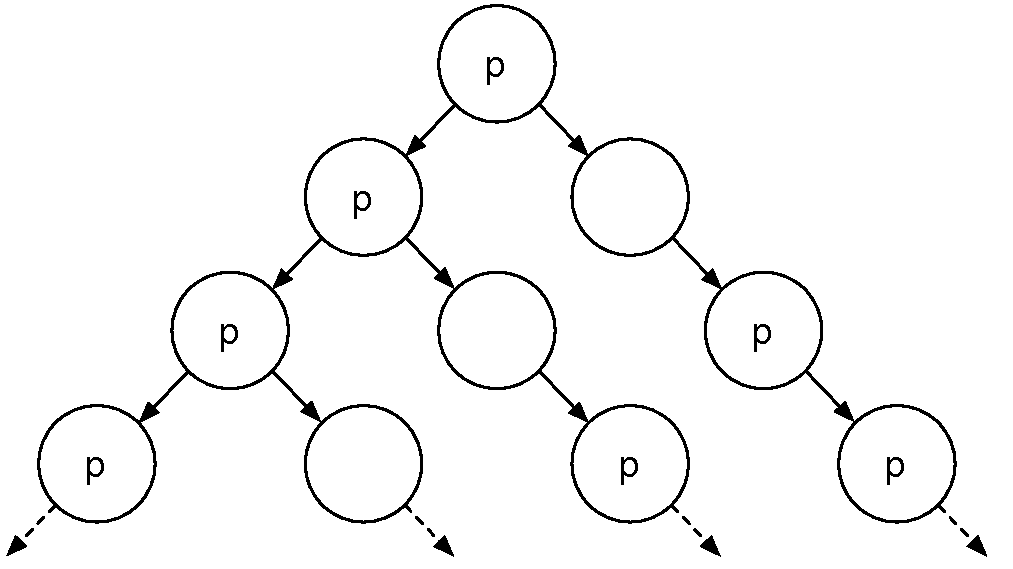
\includegraphics[width=.7\textwidth]
            {Figures/Computation Tree Exercise 6.pdf}
    \caption{Computation Tree for
             Figure~\ref{figure:Kripke_Structure_Exercise_6}}
    \label{figure:Computation_Tree_Exercise_6}
\end{figure}

\begin{description}[style=multiline, leftmargin=3cm]

    \item[$s₀⊧\mathbf{AF}(\mathbf{G}~p)$] This formula specifies that in all
    paths sometimes in the future $p$ will hold globally. This is true for the
    given Kripke structure since we start in $s₀$ in which $p$ holds and either

        \begin{itemize}

            \item continue to stay in this state ($p$ holds globally) or

            \item go to $s₁$ immediately followed by state $s₂$ ($p$ holds
            globally).

        \end{itemize}

    \item[$s₀⊧\mathbf{AF}(\mathbf{AG}~p)$] The formula specifies that
    sometimes in the future for all paths $\mathbf{AG}~p$ (for all paths $p$
    must always be true) has to hold. This is not the case if we follow the
    path on the left in the computation tree for the Kripke Structure (see
    Figure~\ref{figure:Computation_Tree_Exercise_6}) since there is always a
    path on the right where $p$ does not hold for every state.

\end{description}
